\section{Drell-Yan Cross Section Ratio}

\subsection{Extraction of \texorpdfstring{$\bar{d}/\bar{u}$}{dbar/ubar}}
The $\sigma_{pd}/2\sigma_{pp}$ ratio is used by the NNPDF collaboration in 
their PDF extraction\cite{ball2021} and their result is shown in Fig.\ 
\ref{fig:nnpdf_e906}.

\begin{figure}[htbp!]
	\centering
	\begin{subfigure}{0.45\linewidth}
		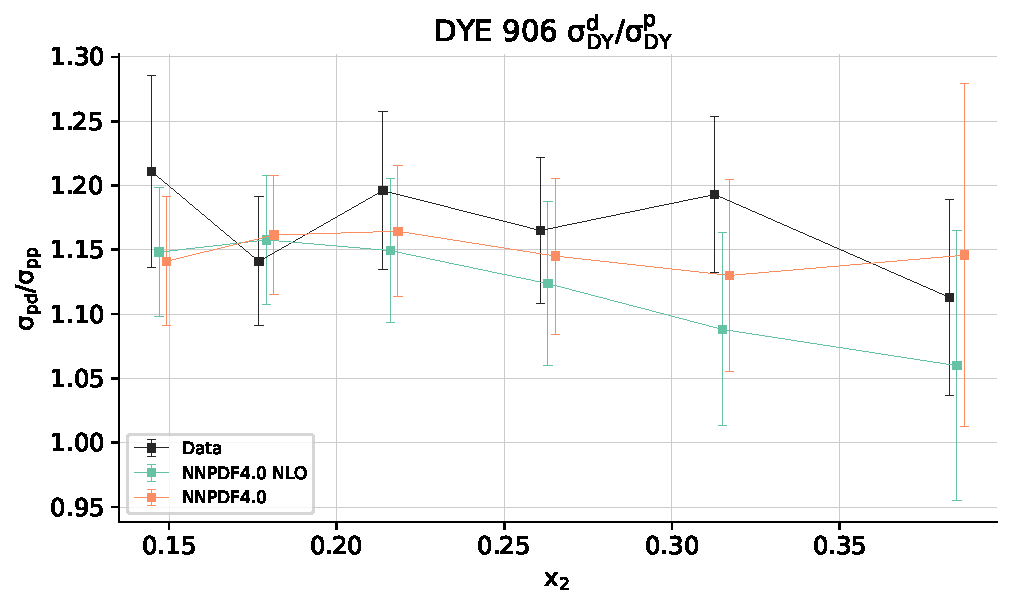
\includegraphics[width=\linewidth]{images/data_vs_theory_nnpdf40_e906}
		\caption{Calculated Drell-Yan cross section ratio.}
		\label{subfig:nnpdf_e906_csr}
	\end{subfigure}
	\begin{subfigure}{0.45\linewidth}
		
\includegraphics[width=\linewidth]{images/placeholder}
		\caption{Extracted $\bar{d/}\bar{u}$ ratio.}
		\label{subfig:nnpdf_e906_x2}
	\end{subfigure}
	\caption{Comparison of NNPDF4.0\cite{ball2021} with the SeaQuest 
	result\cite{dove2021}.}
	\label{fig:nnpdf_e906}
	\pdfmargincomment{Should be compared with the new result from run5-6 and full 
		data set}
\end{figure}

\section{Charmonium Cross Section}
\pdfmargincomment{absolute cross section and cross section ratios; mean pT for
	jpsi as a function of root s}


\subsection{Nuclear Dependence}
